\documentclass[12pt]{article}
\usepackage[capposition=top]{floatrow}
\usepackage{graphicx}
\usepackage{amssymb}
\usepackage{amsmath}
\usepackage{amsfonts}
\usepackage{float}
\usepackage{floatrow}
\usepackage{eurosym}
\usepackage{csvsimple}
\usepackage{booktabs}
\usepackage{tikz}
\usepackage{hyperref}
\usepackage{adjustbox}
\usepackage{ulem}
\usepackage{caption}
\usepackage{tablefootnote}
\usepackage{ntheorem}
\usepackage{sectsty}
\usepackage[justification=centering,textfont={sc},labelfont={rm}]{caption}
\usepackage{geometry}
\geometry{margin=1in}
\usepackage{natbib}
\usepackage{graphicx}
\usepackage{setspace}
\usepackage[section]{placeins}
\onehalfspacing
\begin{document}
	\title{Bringing Expectations to the Collective Bargaining Table: Evidence from Brazilian Firms}
	\author{Valerie R. Boctor\thanks{This project is a collaboration with Roberto Hsu Rocha. This document, including all tables and figures, was written by Valerie Boctor. All mistakes are my own. }}
	\date{\today}
	\maketitle

% =================================================================================================
% 												INTRODUCTION	
% =================================================================================================
	\section{Introduction}
		Using plausibly exogenous variation in the timing of collective bargaining agreements (CBAs) in Brazil, we analyze the effect of an inflationary news shock on firm-level wages and employment. The use of detailed micro data allows us to precisely measure labor market rigidities and the relative bargaining power of firms and workers. Furthermore, we assess the degree of wage rigidity for firms that negotiate just before and just after the inflationary news shock. This research may have important implications for both traditional and expectations-based monetary policy: In particular, we can make inferences about the optimal timing of monetary policy using our precise measure of the time-varying degree of nominal wage rigidity. Additionally, this research may highlight the importance of the collective bargaining channel of expectations-based monetary policy.
	
		\subsection{The Inflationary News Shock}
			 In 2015 Q2, a combination of falling global commodity prices, fiscal malfeasance, and corruption at the state-owned oil company Petrobras sank the Brazilian economy into its deepest recession in over 30 years \cite{yukBrazilSlumpsWorst2016}, \cite{dyerBrazilEconomySlips2015}. Already under fire for ``creative accounting'' on costly social programs during her first term, the newly reelected President Dilma Rousseff became further embroiled when news of her involvement with the Petrobras bribery scheme emerged, solidifying public accusations of vote buying practices, and eroding Brazil's financial capital. Despite having been reprimanded for deferring payment on social programs during her first term,  Dilma Rousseff continued to violate Brazil's budgetary rules, leaving the Bank of Brazil to finance roughly \$4bn without formally issuing a loan \cite{phillipsChargesBrazilianPresident2016}. This practice, known as ``fiscal pedaling'' led to a large increase in government debt and contributed directly to growing inflation rates throughout 2015. Against this backdrop, consumer and business confidence plummeted, reaching their lowest level in 2015 Q3 Figure \ref{fig:BusinessConfidence}, Figure \ref{fig:ConsumerConfidence}. GDP contracted by more than 7\% between 2015 and 2016, while inflation rose steadily from 6.45\% in January 2015 to a high of 9.8\% in June 2016 \cite{leahyCoolHeadCrisis2017}. Taken together, these trends constituted a period of stagflation, not unlike the U.S. experience in the 1970s.

			In a reversal that hearkens back to the Volcker Disinflation, Dilma Rousseff's impeachment and subsequent replacement by Acting President Michael Temer led to significant changes in monetary policy that effectively curbed inflation and set the Brazilian economy on the path to recovery. Michel Temer appointed technocrat Ilan Goldfajn as the Brazilian Central Bank. Goldfajn's credible inflation targeting, interest rate cuts, and reassurance on improved fiscal responsibility helped to stabilize the economy and reduce inflation to under 3.5\% by the close of 2017.

			 We use anticipation of the regime shift as an inflationary news shock. As shown in Figure \ref{fig:Inflation} below, inflation expectations peaked in February 2016 and decline sharply. We attribute the inflection point to a wave of public protests that erupted in March 2016: during that month, a leaked phone-call between Rousseff and her disgraced predecessor, former President Luiz Inácio de Silva, revealed her attempts to shield him from prosecution related to the Petrobras scandal. These protests represented a final push to impeach and a public signal that Rousseff's government would be overturned \cite{douglasReleaseTappedPhone2016}, Figure \ref{fig:Inflation}. It is important to note that speculation of Rousseff's impeachment and potential replacement by Michel Temer (and Ilan Goldfajn) began to appear in the news as early as December 2015, and this messaging was credible and consistent over time. Therefore, it is reasonable to assume the public equated Rousseff's removal from office with the advent of Temer and Goldfajn and an associated reduction in future inflation. 
			 
			\begin{figure}[!ht]
			\centering
			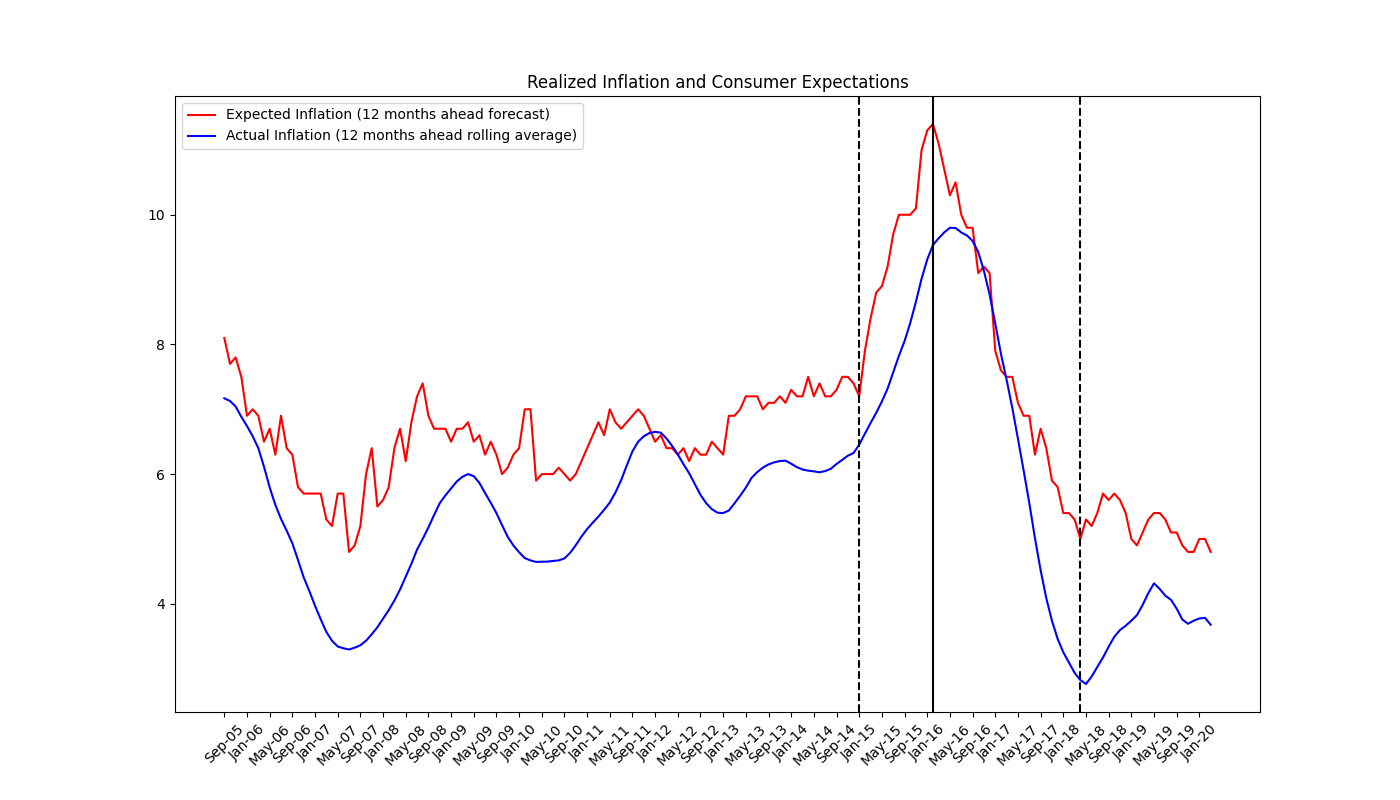
\includegraphics[scale = .5]{tables-figures/Realized_Inflation_and_Consumer_Expectations.png}
			\caption{The inflationary news shock}
			\label{fig:Inflation}
			\floatfoot{Consumer inflation expectations peak in February 2016 and begin to decline thereafter. This timing corresponds to the March 2016, followed by Rousseff's impeachment in April, and suspension of powers in July of the same year.}
			\end{figure}
			
			\begin{figure}[!ht]
				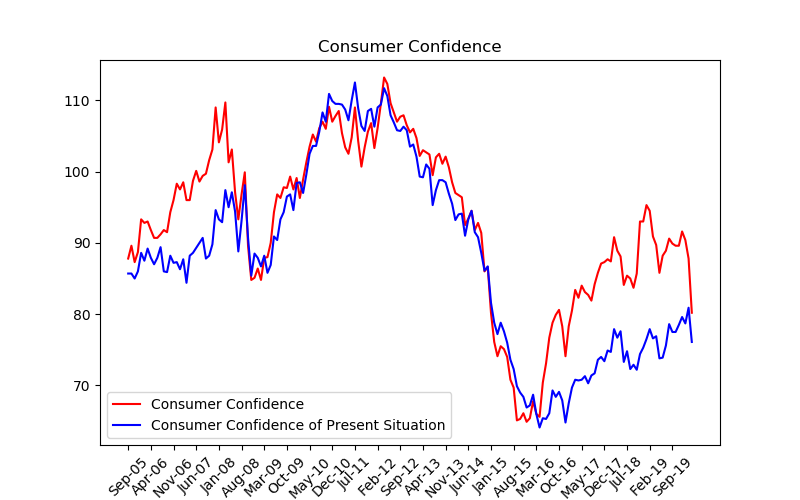
\includegraphics[scale = .8]{old_figures/IBRE_Consumer_Expectations.png}
				\caption{Consumer Confidence Index}
				\floatfoot{Consumer confidence dropped precipitously during the political-economic crisis and began to recover as speculation of Rousseff's replacement by Temer's administration took root.}
				\label{fig:ConsumerConfidence}
			\end{figure}

			\begin{figure}[!ht]
				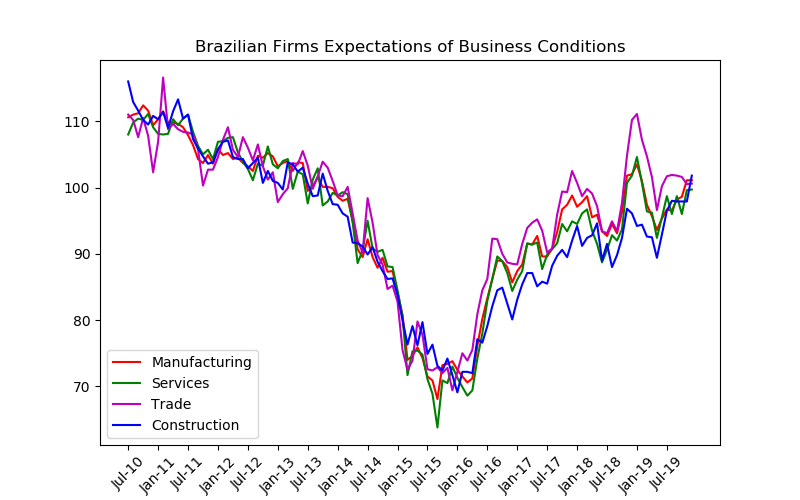
\includegraphics[scale = .85]{old_figures/IBRE_Firm_Expectations.png}
				\caption{Business Confidence Index}
				\label{fig:BusinessConfidence}
				\floatfoot{Business confidence trends across all major sectors strong comovement with consumer confidence, shown in Figure \ref{fig:ConsumerConfidence}.}
			\end{figure} 
 
			\FloatBarrier
		\subsection{Main Research Questions}
		In this project, we are mainly interested in estimating the effect of the inflationary news shock on collective bargaining outcomes in Brazil and understanding macroeconomic implications]. We summarize the main quesstions we will address below:  
		\begin{enumerate}
			\item How does the timing of CBAs affect the response of wages and employment to the inflationary news shock?

			\item To what extent do firm-level wages exhibit nominal rigidities?

			\item What are the implications of wage rigidities and employment behavior for optimal monetary policy?
		\end{enumerate}
% =================================================================================================
% 												BACKGROUND	
% =================================================================================================
	\section{Background}
	In this section, we discuss our intended contributions to the literature and provide key information about collective bargaining institutions in Brazil.
		\subsection{Literature Review}
		Olivei and Tenreyro (2007) posit that monetary policy shocks in the US have larger and less persistent effects during the first and second quarters than in the latter half of the year do to the timing of wage contract negotiations. Because negotiations are more likely to occur in the first two quarters in the US, wages are more flexible during this period and respond more readily to monetary policy shocks. Since wages are less likely to be renegotiated during the third and fourth quarters, the response to monetary policy shocks during these periods tends to be smaller and more protracted. Our research builds on Olivei and Tenreyro's findings by measuring precisely the effect of an aggregate shock on firm-level wages, taking into account the relative timing of each firm's most recent CBA. If the reduction in nominal wages and/or employment is relatviely larger and less persistent for firms CBAs just after the news shock, then our results would corroborate Olivei and Tenreyo's aggregate findings.\footnote{See ``CBAs in Brazil'' for discussion of legally mandated downward nominal wage rigidity and workarounds.}

		% \begin{itemize}
		% 	\item Discuss David Card findings on unions and wage outcomes \cite{cardUnexpectedInflationReal1990}, \cite{cardEffectUnionsStructure1996}, \cite{cardStrikesBargainingSurvey1990}
		% 	\item Discuss relevance to literature on nominal rigidities and macro models \cite{taylorStayingPowerStaggered2016} \cite{taylorChapter15Staggered1999} \cite{fukuiTheoryWageRigidity}
		% \end{itemize}

		\subsection{Collective Bargaining Agreements in Brazil}
		In Brazil, collective bargaining agreements typically last 1 or 2 years. All CBA contracts have a maximum duration of 2 years, but can be extended for additional years. \cite{lagosLaborMarketInstitutions2021} CBAs typically set a fixed nominal wage levels for the duration of the contract. It is important to note that nominal wages are legally required to be downward rigid. That is, nominal wages cannot be reduced unless the union approves the reduction first. Conversely, a reduction in workers' hours must be compensated by a commensurate increase in the nominal wage rate. \cite{EnglishTranslationConsolidation2010}
		
		Given the constraints facing firms, wages (measured in average monthly remuneration) may still be reduced through three main channels: 
		\begin{enumerate}
			\item \textbf{Employment Protection Program} ``Programa de Proteção ao Emprego'' (PPE): This was implemented from July 7, 2015 -  December 31 to protect employment levels during the recession. During this period,  for a maximum of 12 months firms could opt into PPE to temporarily reduce hours by up to 30\% with a proportional reduction in monthly remuneration. The Brazilian government would compensate workers with 50\% of the wage reduction. In our dataset, CBAs involving firms joining PPE begin appearing in 2016, although uptake probably occurred as early as the program start date in July 2015. In future research, it may be interesting to compare wage trends for firms that opted into PPE with those that did not, as well as interactions with collective bargaining activity.
			\item \textbf{separations}: Our measure of wages (average firm-level monthly remuneration) includes the monthly remunerations of workers who separate from the firm mid-month. In effect, mid-month separations would appear in the dataset as a reduction in monthly remuneration. In the future, we will analyze and compare results using a balanced panel of workers from the RAIS data to gauge the importance of the separations channel.
			\item \textbf{reclassifying occupations}: Part of the reduction in average firm-level monthly remuneration may be due to workers being reclassified to occupations with lower implied nominal wages. Similar to the case of separations, reclassifications of this type would register as reductions in wages.
		\end{enumerate}

		In our context, a natural question that arises is whether the frequency and duration of CBAs may be endogenous to inflationary news shocks or changes in economic uncertainty. Below, we present evidence that the timing of CBAs is largely consistent over the entire sample.  
	\begin{figure}[!ht]
		\centering
		\caption{CBA Hazard}
		\label{fig:CBAHazard}	
		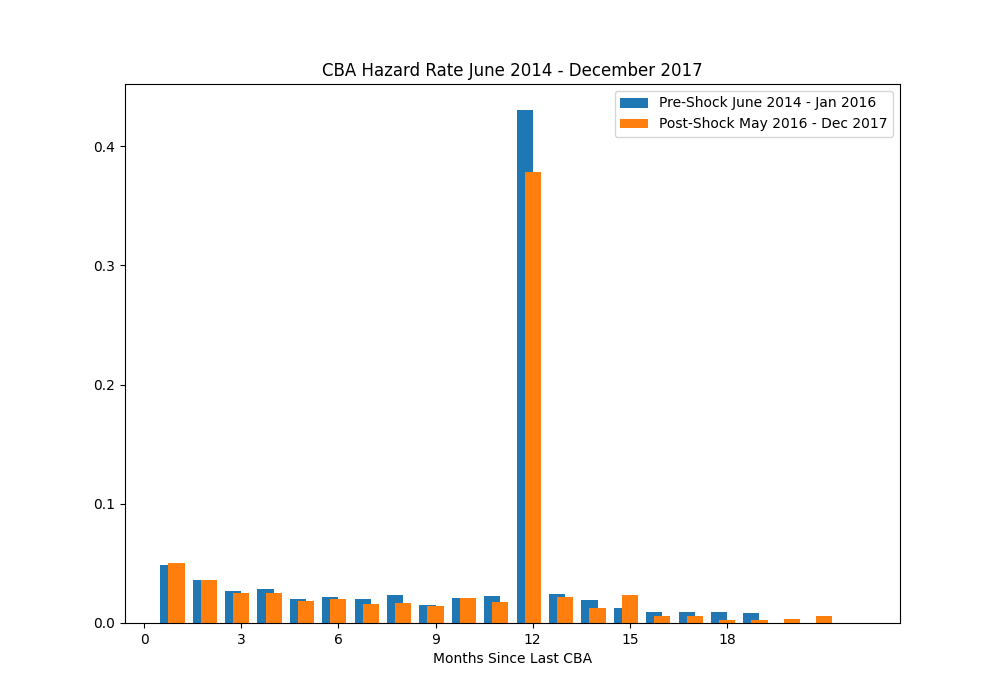
\includegraphics[scale = .72]{tables-figures/cba_hazard.png}
		\floatfoot{The hazard rate for both the pre- and post- shock groups peaks at 12 months.}
		\end{figure}
		Figure \ref{fig:CBAHazard} shows the CBA hazard rate for firms with CBAs before and after the March 2016 shock. For both groups, the hazard rate peaks at 12 months, which suggests that the duration of contracts does not shrink in response to possible uncertainty about future inflation. 

		\begin{figure}[!ht]
			\centering
			\caption{Probability of CBA each period}
			\label{fig:CBAProb}
			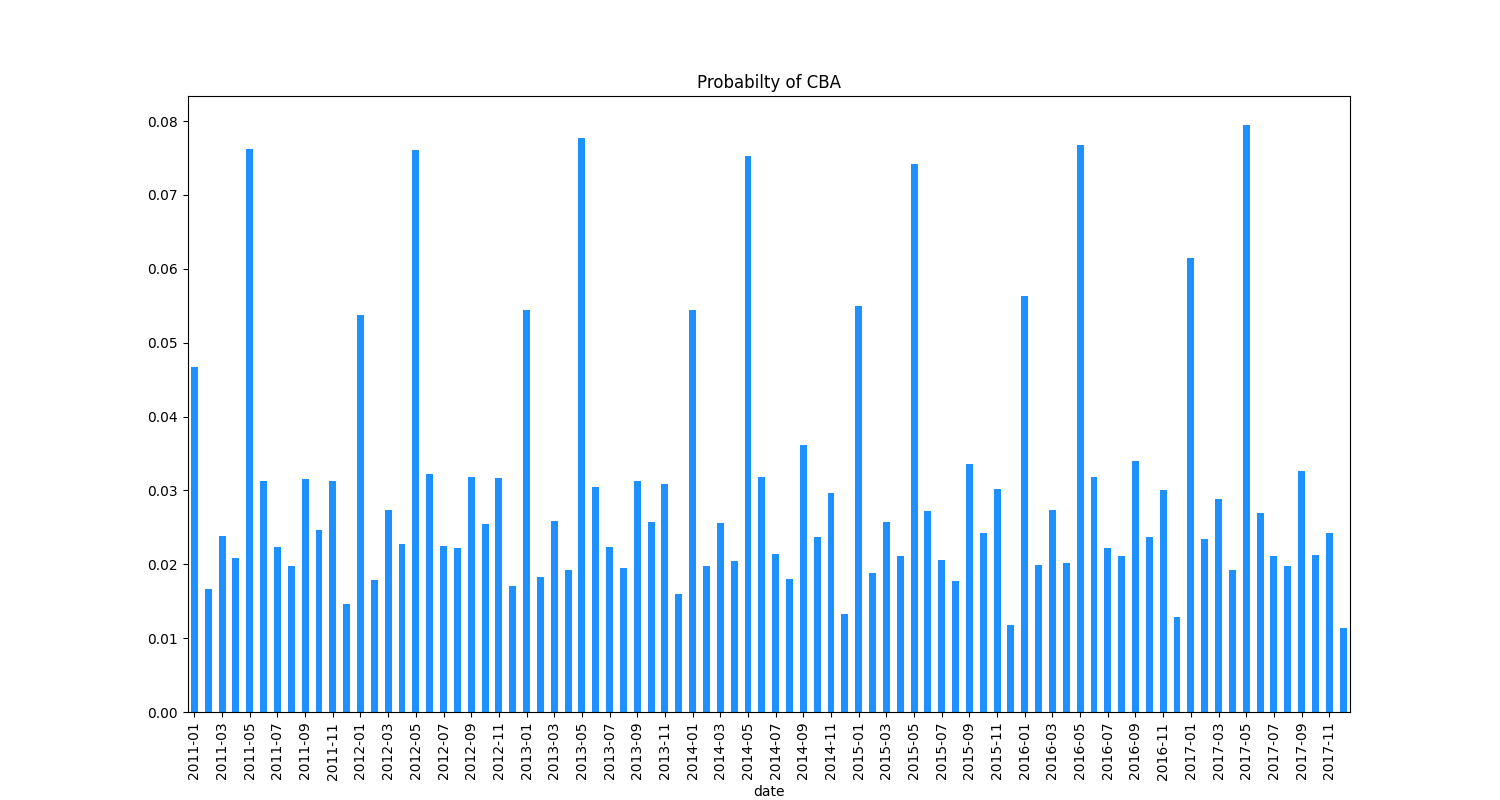
\includegraphics[scale = .5]{tables-figures/cba_probability.png}
			\floatfoot{For each year in the sample, the two most common months for CBAs to occur are January and May. We do not observe changes in the distribution during the 2015-2016 crisis.}
		\end{figure}

		Figure \ref{fig:CBAProb} shows the probability of having a CBA at each period in the sample. Note that the probability of having a CBA does not increase in 2015-2016. This graph suggests that CBAs do not become more frequent in response to news shocks or uncertainty about future inflation.
		Combining information from Figure \ref{fig:CBAHazard} and Figure \ref{fig:CBAProb}, we conclude that the timing of CBAs is plausibly exogenous. 

		Furthermore, we can rule out the possibility that the distribution of CBAs over time is driven by any particular industry. As Lagos (2021) points out, there is no bunching by certain industries around any particular month for CBAs.
% =================================================================================================
% 													DATA	
% =================================================================================================
	\section{Data}
		\subsection{RAIS}
		The Annual Social Information Report (RAIS) is an administrative dataset containing detailed information about workers and employers at the monthly frequency. The key variables of interest are monthly remuneration, employment status, 6-digit occupation codes (CBO), and 2-digit broad sector classifications from IBGE. We use average monthly remuneration by firm as the main wage variable throughout the study. We use the count of employed workers in a given month as the main employment variable of interest. 
		% \begin{figure}
		% 	\centering
		% 	\caption{INSERT RAIS SUM STATS}
		% 	\label{tab:SumStatsRAIS}
		% \end{figure}

		% \begin{figure}
		% 	\centering
		% 	\caption{INSERT RAIS RAW SAMPLE}
		% 	label{tab:RawDataRAIS}
		% \end{figure}

		\subsection{Sistema Mediador}
		Sistema Mediador is the Brazilian Ministry of Labor's online database of all CBAs. We use the subset of collective bargaining agreements that contain individual firm-worker agreements (acordos). This data is webscraped from the Sistema Mediador website. The key variables we use for this study the CBA start and end dates, and company names, which we use to link the CBA data with RAIS.
		% \begin{figure}
		% 	\centering
		% 	\caption{INSERT SM SUM STATS}
		% 	\label{tab:SumStatsRAIS}
		% \end{figure}

		% \begin{figure}
		% 	\centering
		% 	\caption{INSERT SM RAW SAMPLE}
		% 	label{tab:RawDataRAIS}
		% \end{figure} 
		\subsection{FGV IBRE}
		We use aggregate consumer inflation expectations from the Getulio Vargas Foundation (FGV). In the future, we may gain access to firm-specific expectations of their own prices and costs. This information would alllow us to estimate the relationship between expectations and wage adjustments more precisely.
		% \begin{figure}
		% 	\centering
		% 	\caption{INSERT FGV SUM STATS}
		% 	\label{tab:SumStatsRAIS}
		% \end{figure}

		% \begin{figure}
		% 	\centering
		% 	\caption{INSERT FGV RAW SAMPLE}
		% 	label{tab:RawDataRAIS}
		% \end{figure}

% =================================================================================================
% 											EMPIRICAL STRATEGY	
% =================================================================================================
	\section{Research Design}
		\subsection{Reduced Form Model}
		We use the March 16 protests and anticipation of Rousseff's impeachment as the inflationary news shock. We estimate the effects on wages and number of workers over time for firms in the pre- and post- shock groups. We restrict our sample to the subset of firms with contracts beginning either in January 2016 or May 2016. We use January and May 2016 as our pre- and post-shock dates, respectively, for two reasons: 1.)the trajectoryies of average inflation expectations differ substantially across these periods, \footnote{See Figure \ref{fig:Inflation}} and 2.) most CBAs in a given year occur during these months.\footnote{See Figure \ref{fig:CBAProb}} This allows us to take advantage of a substantial part of the variation in the data.
	\begin{align}
		\intertext{We write down the reduced form model for wages as:} \label{eqn:rem_DiD}
		\log{w_{i,t}} & = \alpha_i + \delta_t + \sum_{t=\text{Jan 2015}, t\neq t^{\text{shock}}}^{\text{Dec 2017}} \beta_{t}D_{i,t} + \varepsilon_{i,t} 
		\intertext{Similarly, the model for number of workers is:}  \label{eqn:emp_Did}
		\log{n_{i,t}} & = \alpha_i + \delta_t + \sum_{t=\text{Jan 2015}, t\neq t^{\text{shock}}}^{\text{Dec 2017}} \beta_{t}D_{i,t} + \varepsilon_{i,t} 
	\end{align} 

	In this specification, $D_{i,t}$ is a dummy variable that equals 1 if firm $i$ is in the post-shock group and if the time period of the observation is equal to $t$. A negative estimate for $\beta_t$ would suggest that at time period t, the log wages for firms in the post-shock group fall by more than the pre-shock group. $\alpha_i$ is a firm-level fixed effect, and $\delta_t$ is a time fixed effect for each period in the sample. 

	If wages were perfectly flexible, our prediction, in line with Olivei and Tenreyro (2007), would be that the $\beta_t$ estimates should be most negative just after the shock and attenuate to zero over time. However, for some firms, the presence of legally-required downward rigidity is mitigated by the provisional Employment Protection Program (PPE), which allowed participating firms to temporarily cut hours (and monthly remuneration) by up to 30\%. For firms that did not opt into PPE, a reduction in nominal monthly remuneration is feasible only through separations or by reclassifying workers. (Note that the sample is a balanced panel of firms, so nominal wage reductions cannot be explained by firm exit/entry.) In theory, firms that opted into PPE would use the additional wage flexibility temporarily afforded to behave in a manner more consistent with the predictions of Olivei and Tenyreyro, i.e., cut wages as inflation falls. Participation in PPE represents another form of treatment leading to differential wage flexibility across firms. This potential treatment effect merits study both independently and in connection to the timing of CBAs channel, which we focus on here. 


		\subsection{Preliminary Results}
		\begin{figure}[!ht]
			\centering
			\caption{Monthly Earnings per Worker}
			\label{fig:NormWages}
			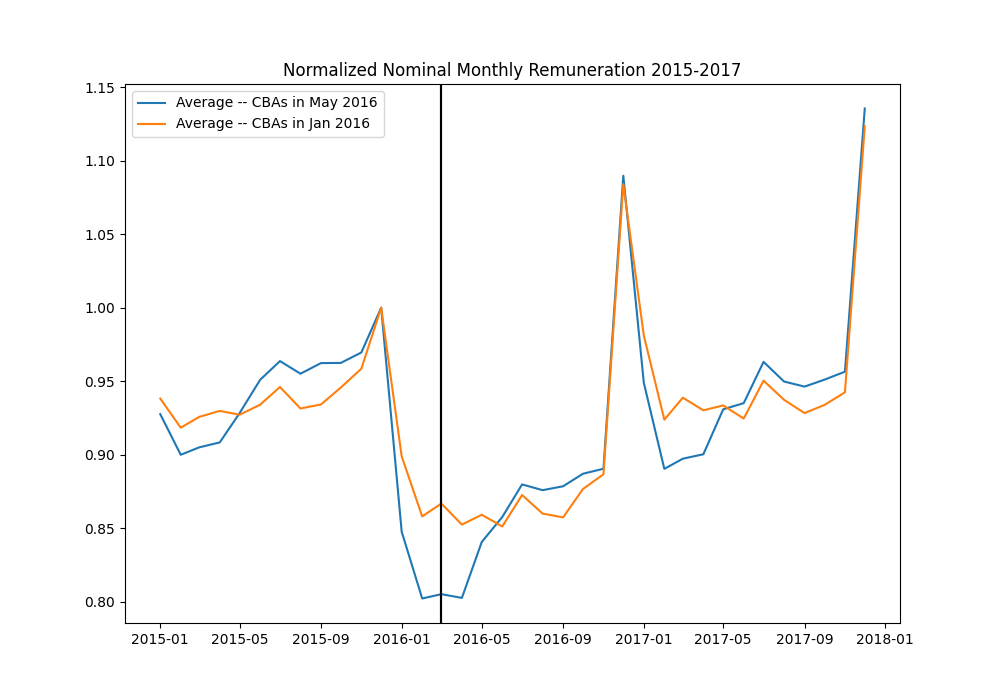
\includegraphics[scale = .65]{tables-figures/normalized_avg_rem_2015_2017.png}
			\floatfoot{Each series is normalized by the values by December 2015 values. The sample is restricted to a balanced panel of firms between 2015 - 2017 with contracts beginning either in January or May 2016. See appendix for figure including median remuneration.}
		\end{figure}
		One of the most striking features of this diagram is the sharp drop in all measures monthly nominal earnings in between December 2015 and January 2016. Surely, part of this drop is due to seasonality: Since bonuses are typically paid out in December, monthly earnings temporarily rise in December and fall back to the trend thereafter. (See November 2016 - January 2017 for comparison). However, the large drop in monthly earnings between December 2015 and January 2016 is salient because wages fall to levels far below the pre-trend levels. While the timing of the drop does not line up with our ``shock'' in March 2016, this graph demonstrates the magnitude of the recession vis-à-vis workers' earnings.  We discuss the difference in nominal wage growth between the pre- and post-shock groups in the regression results in Figure \ref{fig:RegressionResults}.

		\begin{figure}[!ht]
			\centering
			\caption{Number of Workers}
			\label{fig:NormEmp}
			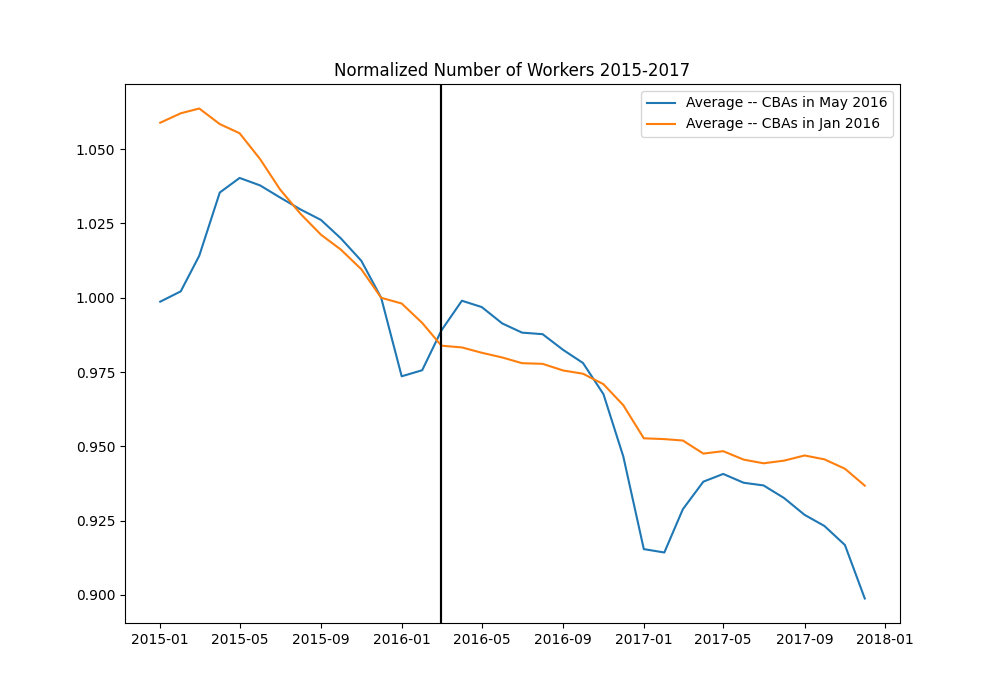
\includegraphics[scale = .65]{tables-figures/normalized_avg_emp_2015_2017.png}
			\floatfoot{Each series is normalized by the values by December 2015 values. The sample is restricted to a balanced panel of firms between 2015 - 2017 with contracts beginning either in January or May 2016 See appendix for figure including median number of workers.}
		\end{figure}
		Next, we present results from the regressions the $\beta_t$ estimates from the difference in differences specifications in equations \ref{eqn:rem_DiD} and  \ref{eqn:emp_Did}. For this analysis, we restrict the sample to a balanced panel of firms between 2015 and 2016 whose contracts begin either in January 2016 or May 2016 and last at least 12 months. Below are the summary statistics for the dataset used in estimation. 

		\begin{table}[!ht]
			\caption{Group Composition by Sector}
			\label{tab:sectors}
			\begin{tabular}{lrrr}
				 & \multicolumn{3}{c}{postshock\_group} \\
Sector&0&1&Total \\
&\%&\%&\% \\
\hline
Administrative Activities and Ancillary Services&12.6&4.6&8.0 \\
Agriculture&1.4&3.3&2.5 \\
Arts, Culture, Sports and Recreation&0.3&1.1&0.8 \\
Construction&3.0&5.9&4.7 \\
Domestic Services&0.0&0.0&0.0 \\
Education&1.0&1.5&1.3 \\
Electricty and Gas&0.3&0.9&0.6 \\
Extractive Industries&0.8&0.7&0.8 \\
Financial Activities and Insurance&5.4&1.0&2.9 \\
Food and Hospitality&3.3&1.7&2.4 \\
Human Health and Social Services&2.9&4.5&3.8 \\
Information and Communication Technologies&2.3&2.0&2.1 \\
International Organizations&0.0&0.0&0.0 \\
Other Services&7.5&11.2&9.6 \\
Processing Industries&34.1&22.0&27.1 \\
Professional, Scientific, and Technical Activities&2.7&2.1&2.3 \\
Public Administratoin, Defense, and Social Security&0.4&0.8&0.6 \\
Real Estate Activities&1.2&0.2&0.6 \\
Sale and Repair of Motor Vehicles &13.7&17.4&15.8 \\
Transport, Storage and Mail&6.3&18.1&13.1 \\
Water and Waste Management&0.9&1.0&1.0 \\
Total&100.0&100.0&100.0 \\

			\end{tabular}
		\end{table}

	\begin{table}[htbp]\centering
\def\sym#1{\ifmmode^{#1}\else\(^{#1}\)\fi}
\caption{DiD Summary Statistics}
\begin{tabular}{l*{2}{c}}
\hline\hline
            &\multicolumn{2}{c}{postshock\_group}\\
            &           0&           1\\
            &     mean/sd&     mean/sd\\
\hline
num\_workers &     193.650&     142.544\\
            &   (637.540)&   (467.514)\\
rem         &    2786.865&    2236.337\\
            &  (2736.130)&  (1784.036)\\
male        &       0.628&       0.670\\
            &     (0.288)&     (0.305)\\
nonwhite    &       0.357&       0.290\\
            &     (0.333)&     (0.318)\\
lesshs      &       0.245&       0.315\\
            &     (0.262)&     (0.295)\\
hs          &       0.479&       0.486\\
            &     (0.283)&     (0.296)\\
morehs      &       0.276&       0.198\\
            &     (0.308)&     (0.272)\\
\hline
\(N\)       &      510264&            \\
\hline\hline
\end{tabular}
\end{table}
[!ht]
		In Figure \ref{fig:NormEmp}, we note that the average and median number of workers per firm is falling during the sample period. This graph provides preliminary evidence that part of the reduction in monthly earnings way be due to separations. 

		 Each point represents the difference in nominal wage growth between firms that negotiated just before the March 2016 shock ($t=0$) and just after.
		\begin{figure}[!ht]
			\centering
			\caption{Response of Nominal Wages and Employment Given CBA Timing}
			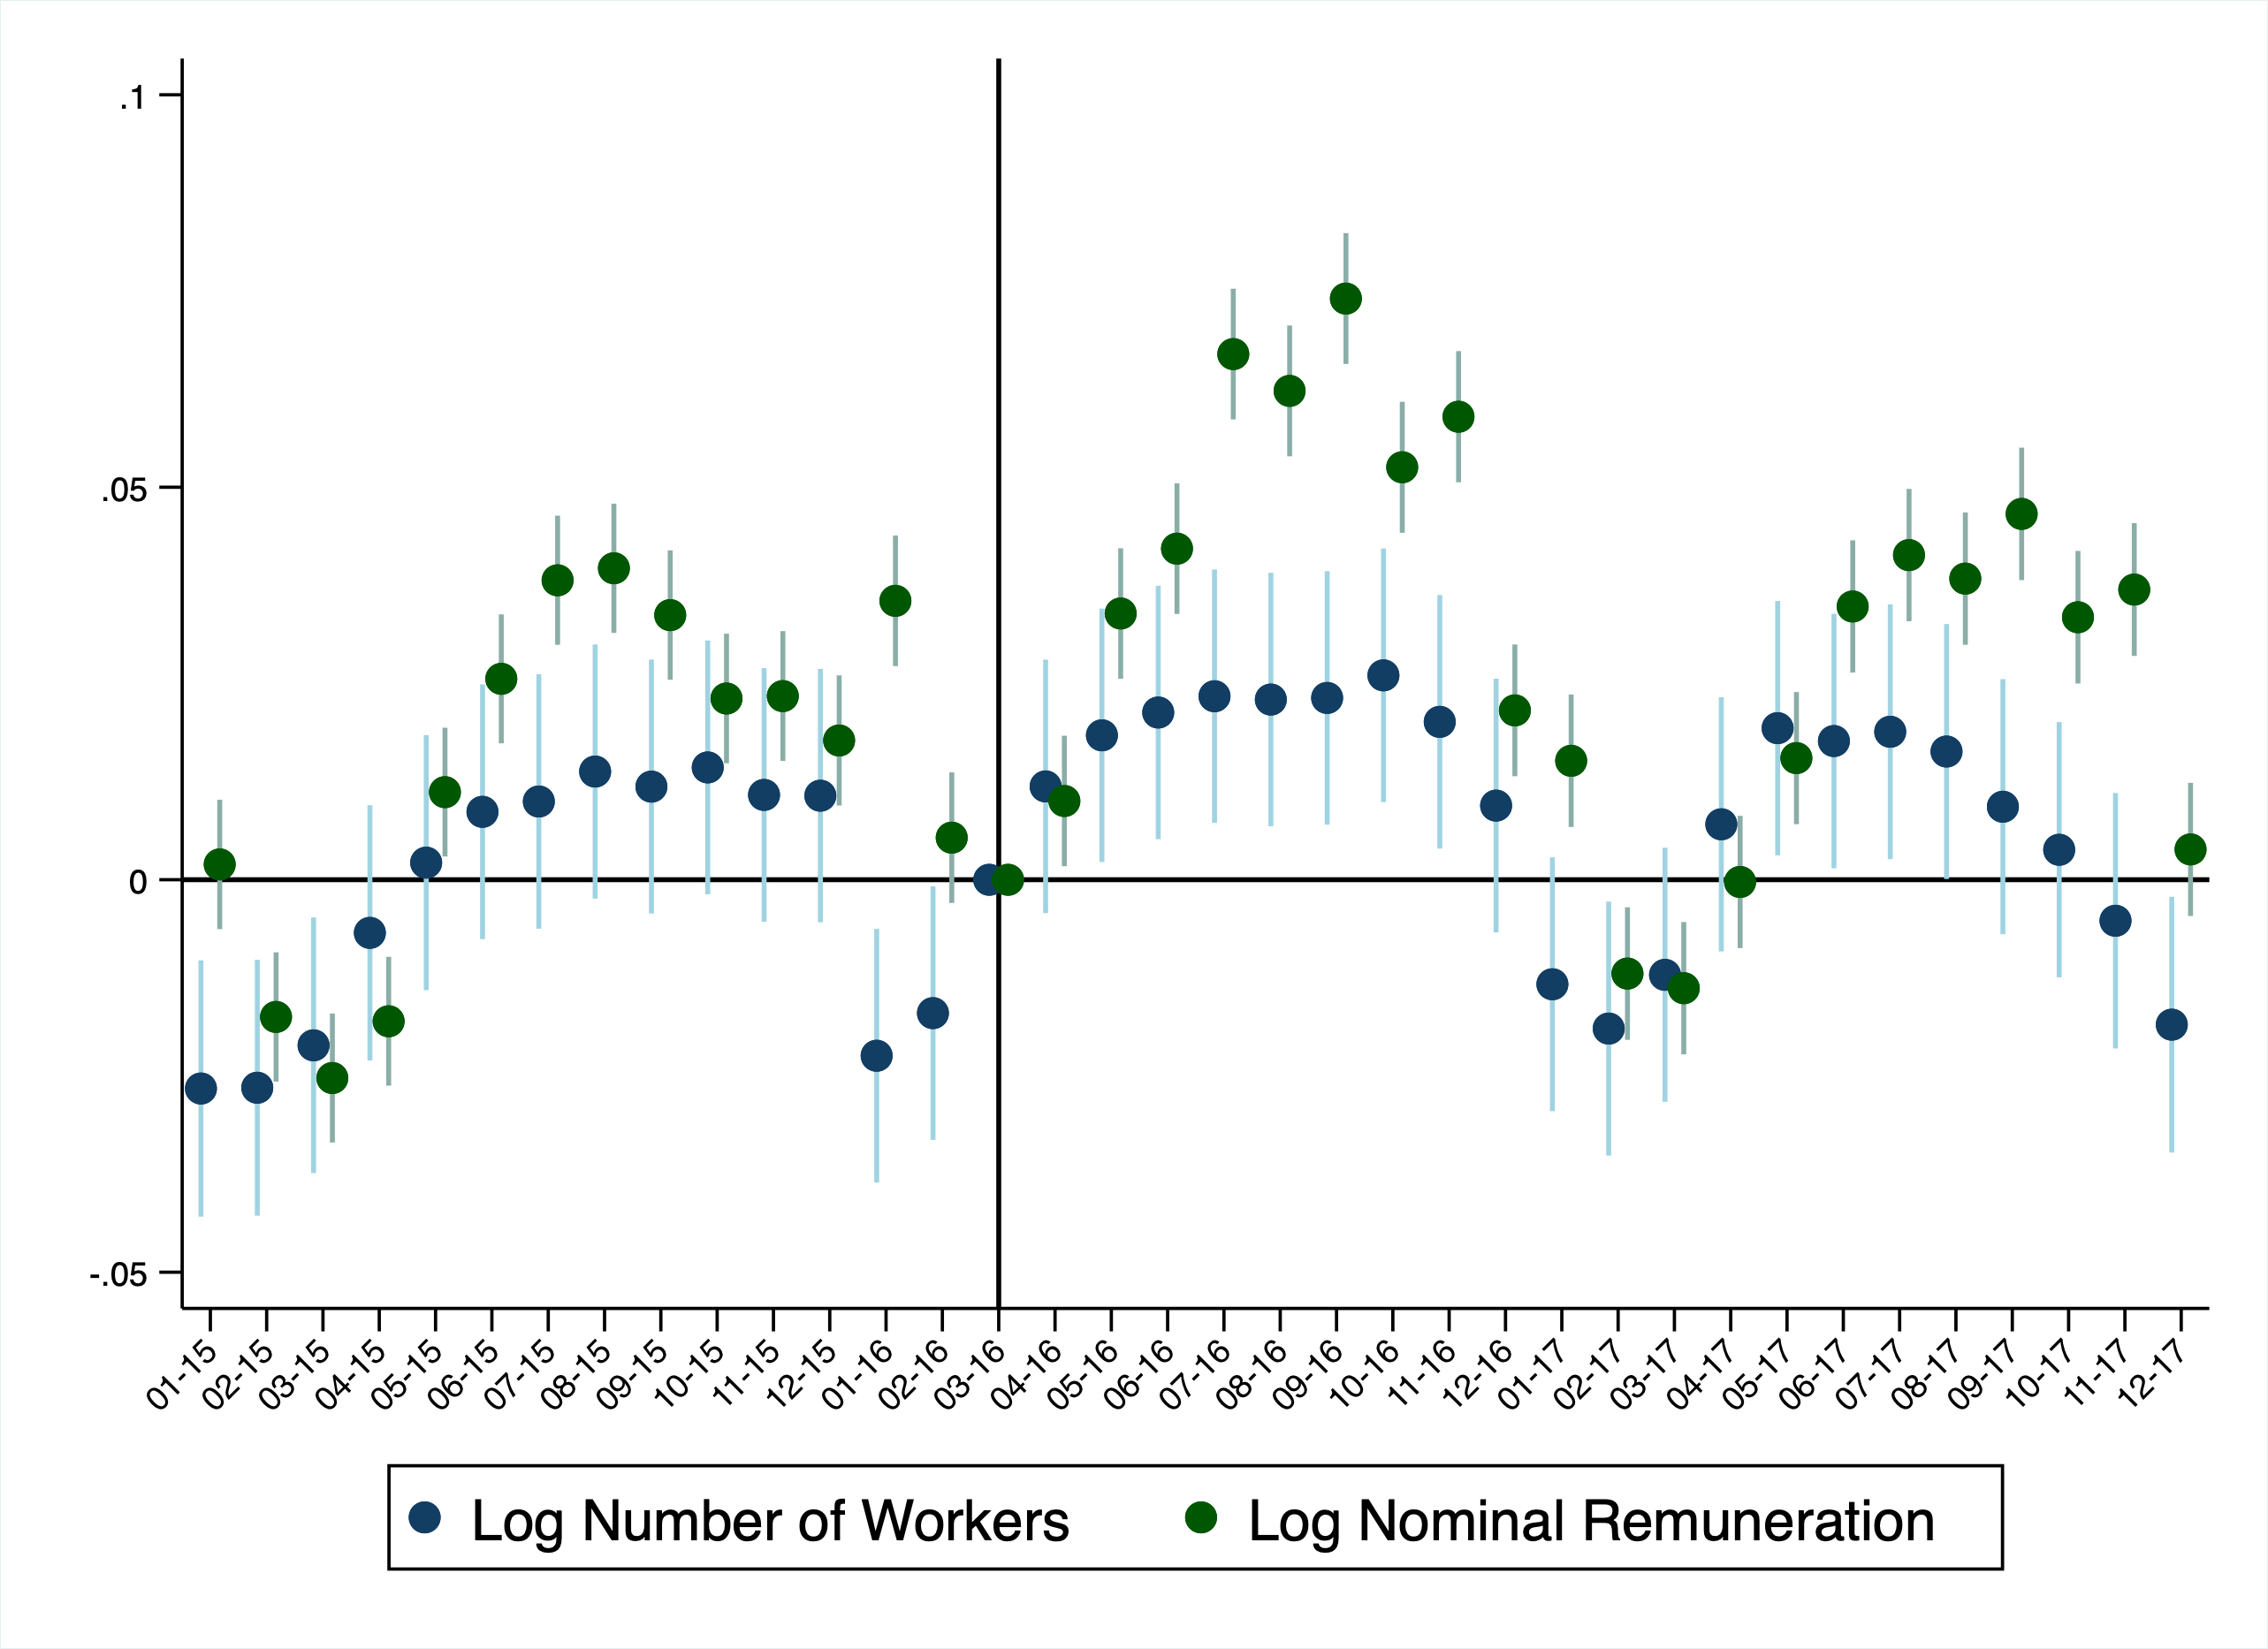
\includegraphics[scale = .375]{tables-figures/DiD_Plots_Weighted_Employment_Rem.png}
			\label{fig:RegressionResults}
			\floatfoot{Regression results from DiD estimation in equations \ref{eqn:emp_Did} and \ref{eqn:rem_DiD}. The results for the wage regressions use analytic weights based on the number of workers at firm $i$ in period $t$. Dashed lines represent when firms in the postshock group would have renegotiations if on a fixed 12-month schedule.}
		\end{figure}
		Contrary to our initial prediction, the DiD results suggest that firms that negotiated contracts just after disinflationary shock had higher nominal wage levels than their counterparts, controlling for time- and firm-level fixed effects. Furthermore, this result is not accompanied by a relative reduction in the number of workers in the post-shock group. Instead, firms in the post-shock exhibit both relatively high nominal wages and employment levels, despite the fact that the real cost to group suggest that the difference in nominal wage growth is statistically indistinguishable from zero until January 2015 (t= -14), represented by the red dashed line on the graph. The coefficients begin to fluctuate after January 2015, as economic uncertainty mounted. The fluctuations become even more pronounced after March 2016 (t=0).


	Tables \ref{tab:wage_reg} and \ref{tab:emp_reg} show several variants of the specifications displayed in Figure \ref{fig:RegressionResults}. 
		\begin{table}[!ht]
				\caption{Log Wage Regressions}
				\label{tab:wage_reg}
				\tiny{{
\def\sym#1{\ifmmode^{#1}\else\(^{#1}\)\fi}
\begin{tabular}{l*{4}{c}}
\hline\hline
          &\multicolumn{1}{c}{(1)}&\multicolumn{1}{c}{(2)}&\multicolumn{1}{c}{(3)}&\multicolumn{1}{c}{(4)}\\
          &\multicolumn{1}{c}{B,W}&\multicolumn{1}{c}{B, NW}&\multicolumn{1}{c}{NB, W}&\multicolumn{1}{c}{NB, NW}\\
\hline
d\_postshock\_14&  0.00195         &   0.0899\sym{***}& 0.000857         &   0.0863\sym{***}\\
          &(0.00420)         & (0.0136)         &(0.00415)         & (0.0136)         \\
d\_postshock\_13&  -0.0175\sym{***}&   0.0852\sym{***}&  -0.0183\sym{***}&   0.0823\sym{***}\\
          &(0.00420)         & (0.0135)         &(0.00415)         & (0.0136)         \\
d\_postshock\_12&  -0.0253\sym{***}&   0.0807\sym{***}&  -0.0267\sym{***}&   0.0768\sym{***}\\
          &(0.00419)         & (0.0135)         &(0.00414)         & (0.0136)         \\
d\_postshock\_11&  -0.0180\sym{***}&   0.0850\sym{***}&  -0.0191\sym{***}&   0.0815\sym{***}\\
          &(0.00419)         & (0.0135)         &(0.00414)         & (0.0135)         \\
d\_postshock\_10&   0.0112\sym{**} &    0.108\sym{***}&   0.0101\sym{*}  &    0.103\sym{***}\\
          &(0.00418)         & (0.0135)         &(0.00413)         & (0.0135)         \\
d\_postshock\_9&   0.0256\sym{***}&    0.120\sym{***}&   0.0237\sym{***}&    0.116\sym{***}\\
          &(0.00419)         & (0.0135)         &(0.00414)         & (0.0135)         \\
d\_postshock\_8&   0.0382\sym{***}&    0.124\sym{***}&   0.0366\sym{***}&    0.120\sym{***}\\
          &(0.00420)         & (0.0135)         &(0.00415)         & (0.0135)         \\
d\_postshock\_7&   0.0397\sym{***}&    0.131\sym{***}&   0.0385\sym{***}&    0.127\sym{***}\\
          &(0.00420)         & (0.0134)         &(0.00415)         & (0.0135)         \\
d\_postshock\_6&   0.0337\sym{***}&    0.132\sym{***}&   0.0325\sym{***}&    0.129\sym{***}\\
          &(0.00421)         & (0.0134)         &(0.00416)         & (0.0135)         \\
d\_postshock\_5&   0.0231\sym{***}&    0.127\sym{***}&   0.0216\sym{***}&    0.124\sym{***}\\
          &(0.00421)         & (0.0134)         &(0.00416)         & (0.0135)         \\
d\_postshock\_4&   0.0234\sym{***}&    0.122\sym{***}&   0.0223\sym{***}&    0.118\sym{***}\\
          &(0.00422)         & (0.0134)         &(0.00417)         & (0.0134)         \\
d\_postshock\_3&   0.0177\sym{***}&    0.114\sym{***}&   0.0151\sym{***}&    0.110\sym{***}\\
          &(0.00423)         & (0.0134)         &(0.00418)         & (0.0134)         \\
d\_postshock\_2&   0.0355\sym{***}&   0.0280\sym{*}  &   0.0348\sym{***}&   0.0259         \\
          &(0.00424)         & (0.0134)         &(0.00419)         & (0.0134)         \\
d\_postshock\_1&  0.00536         &  0.00602         &  0.00609         &  0.00329         \\
          &(0.00425)         & (0.0134)         &(0.00419)         & (0.0134)         \\
d\_postshock0&        0         &        0         &        0         &        0         \\
          &      (.)         &      (.)         &      (.)         &      (.)         \\
d\_postshock1&   0.0100\sym{*}  & 0.000667         &  0.00920\sym{*}  &-0.000240         \\
          &(0.00424)         & (0.0134)         &(0.00418)         & (0.0134)         \\
d\_postshock2&   0.0339\sym{***}&   0.0495\sym{***}&   0.0330\sym{***}&   0.0504\sym{***}\\
          &(0.00424)         & (0.0134)         &(0.00419)         & (0.0134)         \\
d\_postshock3&   0.0422\sym{***}&   0.0871\sym{***}&   0.0425\sym{***}&   0.0875\sym{***}\\
          &(0.00425)         & (0.0134)         &(0.00419)         & (0.0134)         \\
d\_postshock4&   0.0670\sym{***}&   0.0946\sym{***}&   0.0661\sym{***}&   0.0934\sym{***}\\
          &(0.00425)         & (0.0134)         &(0.00420)         & (0.0134)         \\
d\_postshock5&   0.0623\sym{***}&    0.104\sym{***}&   0.0618\sym{***}&   0.0998\sym{***}\\
          &(0.00425)         & (0.0134)         &(0.00420)         & (0.0134)         \\
d\_postshock6&   0.0740\sym{***}&    0.117\sym{***}&   0.0727\sym{***}&    0.115\sym{***}\\
          &(0.00425)         & (0.0134)         &(0.00420)         & (0.0134)         \\
d\_postshock7&   0.0525\sym{***}&    0.101\sym{***}&   0.0518\sym{***}&    0.104\sym{***}\\
          &(0.00426)         & (0.0134)         &(0.00421)         & (0.0134)         \\
d\_postshock8&   0.0590\sym{***}&   0.0861\sym{***}&   0.0580\sym{***}&   0.0807\sym{***}\\
          &(0.00426)         & (0.0134)         &(0.00421)         & (0.0134)         \\
d\_postshock9&   0.0216\sym{***}&    0.110\sym{***}&   0.0203\sym{***}&    0.105\sym{***}\\
          &(0.00428)         & (0.0134)         &(0.00423)         & (0.0134)         \\
d\_postshock10&   0.0152\sym{***}&   0.0524\sym{***}&   0.0138\sym{**} &   0.0487\sym{***}\\
          &(0.00431)         & (0.0134)         &(0.00427)         & (0.0135)         \\
d\_postshock11&  -0.0120\sym{**} &   0.0273\sym{*}  &  -0.0130\sym{**} &   0.0254         \\
          &(0.00431)         & (0.0134)         &(0.00427)         & (0.0135)         \\
d\_postshock12&  -0.0138\sym{**} &   0.0240         &  -0.0153\sym{***}&   0.0207         \\
          &(0.00430)         & (0.0134)         &(0.00426)         & (0.0135)         \\
d\_postshock13&-0.000283         &   0.0288\sym{*}  & -0.00173         &   0.0236         \\
          &(0.00430)         & (0.0134)         &(0.00426)         & (0.0135)         \\
d\_postshock14&   0.0155\sym{***}&   0.0661\sym{***}&   0.0146\sym{***}&   0.0640\sym{***}\\
          &(0.00429)         & (0.0135)         &(0.00425)         & (0.0135)         \\
d\_postshock15&   0.0348\sym{***}&   0.0842\sym{***}&   0.0337\sym{***}&   0.0809\sym{***}\\
          &(0.00430)         & (0.0135)         &(0.00426)         & (0.0135)         \\
d\_postshock16&   0.0414\sym{***}&   0.0922\sym{***}&   0.0403\sym{***}&   0.0887\sym{***}\\
          &(0.00430)         & (0.0135)         &(0.00426)         & (0.0135)         \\
d\_postshock17&   0.0384\sym{***}&    0.102\sym{***}&   0.0373\sym{***}&   0.0988\sym{***}\\
          &(0.00430)         & (0.0135)         &(0.00426)         & (0.0136)         \\
d\_postshock18&   0.0466\sym{***}&   0.0988\sym{***}&   0.0454\sym{***}&   0.0967\sym{***}\\
          &(0.00430)         & (0.0135)         &(0.00426)         & (0.0136)         \\
d\_postshock19&   0.0334\sym{***}&   0.0871\sym{***}&   0.0324\sym{***}&   0.0827\sym{***}\\
          &(0.00431)         & (0.0135)         &(0.00427)         & (0.0136)         \\
d\_postshock20&   0.0370\sym{***}&   0.0896\sym{***}&   0.0362\sym{***}&   0.0882\sym{***}\\
          &(0.00431)         & (0.0135)         &(0.00427)         & (0.0136)         \\
d\_postshock21&  0.00387         &    0.104\sym{***}&  0.00254         &   0.0989\sym{***}\\
          &(0.00433)         & (0.0135)         &(0.00429)         & (0.0136)         \\
\hline
\(N\)     &   501229         &   501229         &   517654         &   517654         \\
\hline\hline
\multicolumn{5}{l}{\footnotesize Standard errors in parentheses}\\
\multicolumn{5}{l}{\footnotesize Dependent variable is log of monthly remuneration}\\
\multicolumn{5}{l}{\footnotesize \sym{*} \(p<0.05\), \sym{**} \(p<0.01\), \sym{***} \(p<0.001\)}\\
\end{tabular}
}
}
				\floatfoot{B/ NB = Balanced/ Unbalanced, W/ NW = Weighted/ Unweighted. \\ Weights are based on number of workers at firm $i$ in period $t$.}
		\end{table}

		\begin{table}[!ht]
			\caption{Log Employment Regressions}
			\label{tab:emp_reg}
			\tiny{{
\def\sym#1{\ifmmode^{#1}\else\(^{#1}\)\fi}
\begin{tabular}{l*{2}{c}}
\hline\hline
          &\multicolumn{1}{c}{(1)}&\multicolumn{1}{c}{(2)}\\
          &\multicolumn{1}{c}{B}&\multicolumn{1}{c}{NB}\\
\hline
d\_postshock\_14&  -0.0125         &  -0.0219\sym{*}  \\
          &(0.00903)         &(0.00851)         \\
d\_postshock\_13&  -0.0124         &  -0.0185\sym{*}  \\
          &(0.00901)         &(0.00850)         \\
d\_postshock\_12& -0.00793         &  -0.0158         \\
          &(0.00900)         &(0.00848)         \\
d\_postshock\_11&  0.00551         & -0.00157         \\
          &(0.00899)         &(0.00847)         \\
d\_postshock\_10&   0.0148         &  0.00787         \\
          &(0.00898)         &(0.00848)         \\
d\_postshock\_9&   0.0199\sym{*}  &   0.0128         \\
          &(0.00898)         &(0.00845)         \\
d\_postshock\_8&   0.0207\sym{*}  &   0.0141         \\
          &(0.00896)         &(0.00844)         \\
d\_postshock\_7&   0.0232\sym{**} &   0.0195\sym{*}  \\
          &(0.00895)         &(0.00842)         \\
d\_postshock\_6&   0.0223\sym{*}  &   0.0186\sym{*}  \\
          &(0.00895)         &(0.00842)         \\
d\_postshock\_5&   0.0250\sym{**} &   0.0221\sym{**} \\
          &(0.00894)         &(0.00841)         \\
d\_postshock\_4&   0.0190\sym{*}  &   0.0184\sym{*}  \\
          &(0.00893)         &(0.00841)         \\
d\_postshock\_3&   0.0153         &   0.0166\sym{*}  \\
          &(0.00893)         &(0.00840)         \\
d\_postshock\_2&  -0.0237\sym{**} &  -0.0165\sym{*}  \\
          &(0.00893)         &(0.00838)         \\
d\_postshock\_1&  -0.0189\sym{*}  &  -0.0166\sym{*}  \\
          &(0.00893)         &(0.00839)         \\
d\_postshock0&        0         &        0         \\
          &      (.)         &      (.)         \\
d\_postshock1&   0.0132         &   0.0138         \\
          &(0.00893)         &(0.00838)         \\
d\_postshock2&   0.0213\sym{*}  &   0.0278\sym{***}\\
          &(0.00892)         &(0.00837)         \\
d\_postshock3&   0.0256\sym{**} &   0.0341\sym{***}\\
          &(0.00892)         &(0.00837)         \\
d\_postshock4&   0.0255\sym{**} &   0.0346\sym{***}\\
          &(0.00892)         &(0.00837)         \\
d\_postshock5&   0.0255\sym{**} &   0.0335\sym{***}\\
          &(0.00892)         &(0.00837)         \\
d\_postshock6&   0.0249\sym{**} &   0.0321\sym{***}\\
          &(0.00893)         &(0.00838)         \\
d\_postshock7&   0.0277\sym{**} &   0.0351\sym{***}\\
          &(0.00893)         &(0.00839)         \\
d\_postshock8&   0.0227\sym{*}  &   0.0285\sym{***}\\
          &(0.00893)         &(0.00839)         \\
d\_postshock9&  0.00923         &   0.0183\sym{*}  \\
          &(0.00894)         &(0.00841)         \\
d\_postshock10&  -0.0135         & -0.00840         \\
          &(0.00894)         &(0.00845)         \\
d\_postshock11&  -0.0202\sym{*}  &  -0.0137         \\
          &(0.00894)         &(0.00845)         \\
d\_postshock12&  -0.0119         & -0.00453         \\
          &(0.00895)         &(0.00845)         \\
d\_postshock13&  0.00698         &   0.0148         \\
          &(0.00895)         &(0.00845)         \\
d\_postshock14&   0.0197\sym{*}  &   0.0267\sym{**} \\
          &(0.00896)         &(0.00846)         \\
d\_postshock15&   0.0185\sym{*}  &   0.0244\sym{**} \\
          &(0.00896)         &(0.00847)         \\
d\_postshock16&   0.0192\sym{*}  &   0.0255\sym{**} \\
          &(0.00897)         &(0.00847)         \\
d\_postshock17&   0.0158         &   0.0248\sym{**} \\
          &(0.00898)         &(0.00847)         \\
d\_postshock18&  0.00946         &   0.0166         \\
          &(0.00898)         &(0.00848)         \\
d\_postshock19&  0.00384         &   0.0103         \\
          &(0.00899)         &(0.00849)         \\
d\_postshock20& -0.00566         &  0.00131         \\
          &(0.00900)         &(0.00850)         \\
d\_postshock21&  -0.0184\sym{*}  &  -0.0113         \\
          &(0.00901)         &(0.00850)         \\
\_cons    &    3.383\sym{***}&    3.426\sym{***}\\
          &(0.00383)         &(0.00347)         \\
\hline
\(N\)     &   442253         &   504441         \\
\hline\hline
\multicolumn{3}{l}{\footnotesize Standard errors in parentheses}\\
\multicolumn{3}{l}{\footnotesize Dependent variable is log of number of workers}\\
\multicolumn{3}{l}{\footnotesize \sym{*} \(p<0.05\), \sym{**} \(p<0.01\), \sym{***} \(p<0.001\)}\\
\end{tabular}
}
}
			\floatfoot{B/ NB = Balanced/ Unbalanced}
		\end{table}

% =================================================================================================
% 													THEORY	
% =================================================================================================
	\section{Future Research}
	Further analysis is required to pin down what factors are driving the reduction in nominal wages across all firms during the 2015-2016 recession.\footnote{See Figure \ref{fig:NormWages}} One possible explanation is that a large share of firms may be opting into PPE, as discussed above. Another possible explanation is that firms separate from workers at a higher rate during the recession, curtailing the workers' monthly earnings. There is some preliminary evidence of this in Figure \ref{fig:NormEmp}. Another potentially complementary explanation is that firms reclassify workers to occupations with lower implied nominal wages. While we have not yet carried out the analyses to distinguish between these explanations, we may have sufficient data to accomplish this in the near future.

	Furthermore, the sheer size in the drop of nominal monthly remuneration during the recession across CBA groups suggests that it may be beneficial to broaden the scope our research beyond the inflationary news shock narrative to focus on the labor market effects of the recession as a whole. Relatedly, it may beneficial to reconsider whether the standard predictions of macro models (i.e., inflation and GDP are positively correlated) are applicable to the Brazilian context in 2015-2016. \cite{goncalvesAssessingBrazilianMacroeconomic2016a} find that during periods of high volatility in Brazil, inflation and output are negatively correlated. If this is true for the 2015-2016 recession, our predictions for the direction of wage and employment  variables in response to the disinflationary news may not necessarily align with the findings of Olivei and Tenreyro. An interesting question is what the model-based implications for the direction of wages and employment during a high volatility period would be, and whether these predictions hold empirically.

	Another salient question is why firms that negotiate wages just after the shock set higher nominal wages than firms negotiating just before Figure \ref{fig:RegressionResults}. An important piece of this puzzle could be that the result is driven by particular sectors, or by potential cyclicality in the bargaining power of workers, particularly in the post-shock group. While we do not currently have evidence this is the case, further work is required to corroborate this empirically. Another possible explanation is that firms in the post-shock group have higher levels of optimism about the future state of the economy and their own future profit margins, which may lead them to set higher wage levels. We may gain access to microdata on firms' own-price and own-cost expectations that would allow us to study the link between individual firms' expectations and negotiated wages as well as hiring and firing decisions.  

	In a later stage of the paper, we plan to use a structural model to rationalize our empirical findings. For example, following Olivei and Tenreyo (2007), we may adapt a dynamic stochastic general equilibrium model with uneven staggering of wage contracts and downward rigidity. Another approach would be to adapt a DMP model to include inflation expectations. \cite{fukuiTheoryWageRigidity2020}

\section{Appendix}
	\begin{figure}[!ht]
		\centering
		\caption {Typical CBA in Sistema Mediador}
		\label{typical_CBA}
		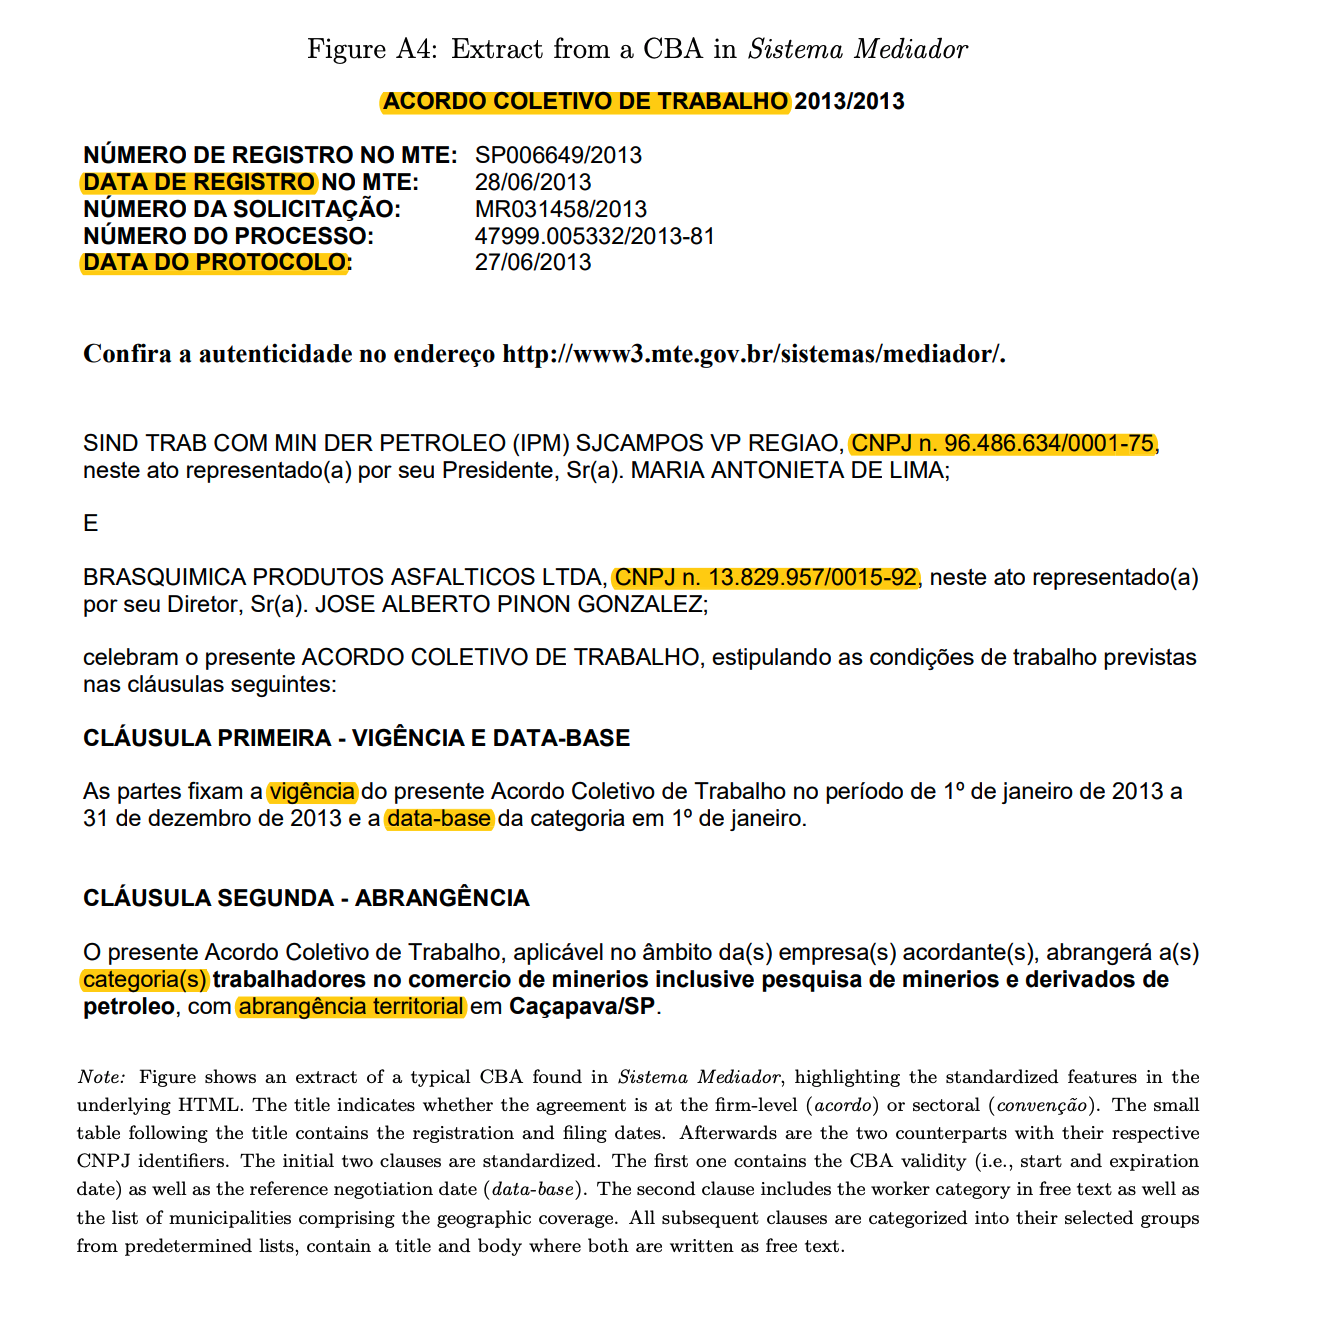
\includegraphics[scale=.6]{tables-figures/Typical_CBA.png}
		\floatfoot{Excerpt from \cite{lagosLaborMarketInstitutions2021}.}
	\end{figure}
	\begin{figure}[!ht]
		\centering
		\caption{Monthly Earnings per Worker}
		\label{fig:NormWages_Med}
		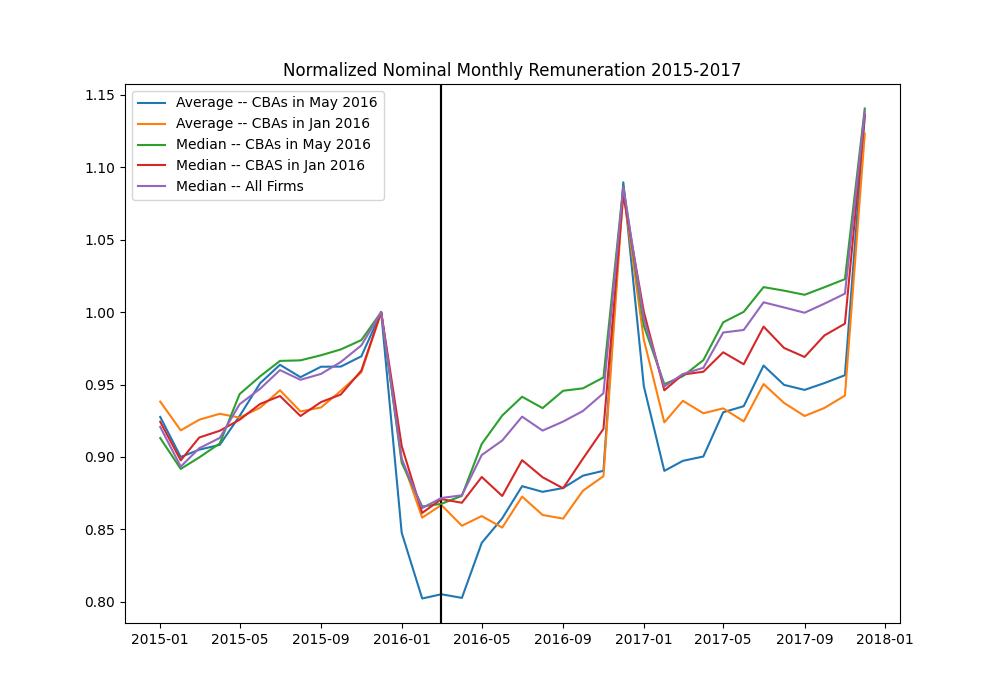
\includegraphics[scale = .65]{tables-figures/normalized_avg_med_rem_2015_2017.png}
		\floatfoot{Each series is normalized by the values by December 2015 values. The sample is restricted to a balanced panel of firms between 2015 - 2017 with contracts beginning either in January or May 2016.}
	\end{figure}

	\begin{figure}[!ht]
		\centering
		\caption{Number of Workers}
		\label{fig:NormEmp_Med}	
		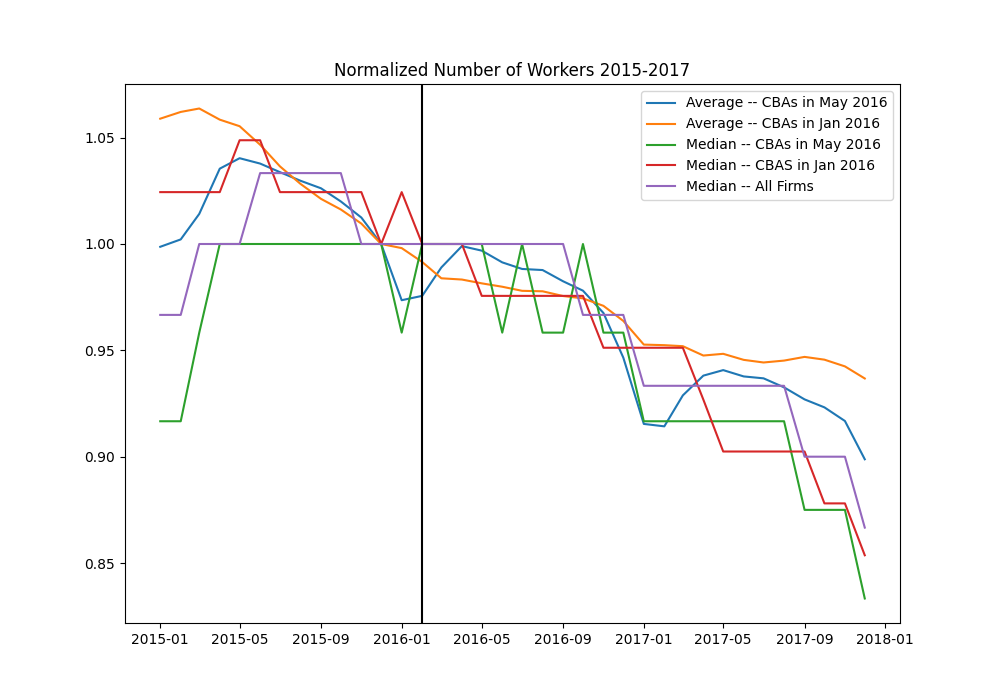
\includegraphics[scale = .65]{tables-figures/normalized_avg_med_emp_2015_2017.png}
		\floatfoot{Each series is normalized by the values by December 2015 values. The sample is restricted to a balanced panel of firms between 2015 - 2017 with contracts beginning either in January or May 2016.}
		\end{figure}
% =================================================================================================
% 												FUTURE RESEARCH	
% =================================================================================================

	\newpage
	\bibliographystyle{chicago}
	\bibliography{Bibliography-CBAs-Inflation}
	\end{document}